\begin{flushright} {\tiny {\color{gray} basis\_p4\_2D.tex}} \end{flushright}
%~~~~~~~~~~~~~~~~~~~~~~~~~~~~~~~~~~~~~~~~~~~~~~~~~~~~~~~~~~~~~~~~~~~~~~~~~~~~~~~~~~~~~~~~~~~~~~~~~~

It is implemented in \stone~120.
See also python code in {\tt images/basis\_P4} which I wrote to test these basis functions.

\begin{flushright} {\tiny {\color{gray} (tikz\_p4.tex)}} \end{flushright}
%~~~~~~~~~~~~~~~~~~~~~~~~~~~~~~~~~~~~~~~~~~~~~~~~~~~~~~~~~~~~~~~~~~~~~~~~~~~~~~~~~~~~~~~~~~~~~~~~~~

\begin{center}
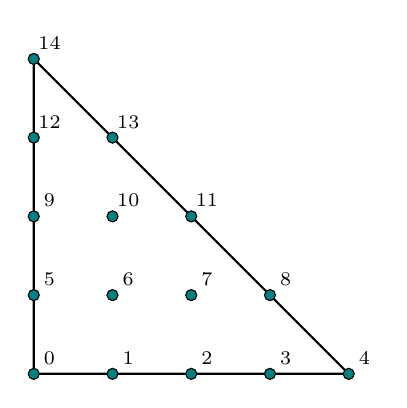
\begin{tikzpicture}
%\draw[step=0.5cm,gray,very thin] (0,0) grid (5,3.5); %bckgr grid
\draw[thick] (0,0) -- (4,0)  -- (0,4) -- cycle; 

\draw[black,fill=teal] (0,0) circle (2pt);
\draw[black,fill=teal] (1,0) circle (2pt);
\draw[black,fill=teal] (2,0) circle (2pt);
\draw[black,fill=teal] (3,0) circle (2pt);
\draw[black,fill=teal] (4,0) circle (2pt);
\draw[black,fill=teal] (0,1) circle (2pt);
\draw[black,fill=teal] (1,1) circle (2pt);
\draw[black,fill=teal] (2,1) circle (2pt);
\draw[black,fill=teal] (3,1) circle (2pt);
\draw[black,fill=teal] (0,2) circle (2pt);
\draw[black,fill=teal] (1,2) circle (2pt);
\draw[black,fill=teal] (2,2) circle (2pt);
\draw[black,fill=teal] (0,3) circle (2pt);
\draw[black,fill=teal] (1,3) circle (2pt);
\draw[black,fill=teal] (0,4) circle (2pt);

\node[] at (0.2,0.2) {\scriptsize $0$};
\node[] at (1.2,0.2) {\scriptsize $1$};
\node[] at (2.2,0.2) {\scriptsize $2$};
\node[] at (3.2,0.2) {\scriptsize $3$};
\node[] at (4.2,0.2) {\scriptsize $4$};
\node[] at (0.2,1.2) {\scriptsize $5$};
\node[] at (1.2,1.2) {\scriptsize $6$};
\node[] at (2.2,1.2) {\scriptsize $7$};
\node[] at (3.2,1.2) {\scriptsize $8$};
\node[] at (0.2,2.2) {\scriptsize $9$};
\node[] at (1.2,2.2) {\scriptsize $10$};
\node[] at (2.2,2.2) {\scriptsize $11$};
\node[] at (0.2,3.2) {\scriptsize $12$};
\node[] at (1.2,3.2) {\scriptsize $13$};
\node[] at (0.2,4.2) {\scriptsize $14$};

\end{tikzpicture}
\end{center}


The support nodes coordinates are as follows:

\begin{center}
\begin{tabular}{cccccccccccccccc}
\hline
$i\rightarrow$& 0& 1 &2 &3 &4 &5 &6 &7 &8 &9 &10 &11 &12 &13 &14  \\
\hline\hline
$r_i$&0&$\frac14$ & $\frac12$ & $\frac34$ & 1 &0 &$\frac14$&$\frac12$&
$\frac34$&0&$\frac14$&$\frac12$&0&$\frac14$&0    \\
$s_i$&0&0&0&0&0&$\frac14$&$\frac14$&$\frac14$&$\frac14$
&$\frac12$&$\frac12$&$\frac12$
&$\frac34$&$\frac34$&1\\
\hline
\end{tabular}
\end{center}

Inside the element a field $f$ is represented by a 4-th order polynomial:
\begin{eqnarray}
f^h(r,s)
&=&c_0 + c_1 r+c_2 s \nn\\
&&+ c_3 r^2 + c_4 rs + c_5 s^2 \nn\\
&&+c_6r^3 + c_7 r^2s + c_8 rs^2 + c_9 s^3 \nn\\
&&
+ c_{10} r^4 
+ c_{11} r^3s 
+ c_{12} r^2s^2
+ c_{13} rs^3
+c_{14} s^4
\end{eqnarray}

At each node the function takes a value $f_i$, $i\in[0,14]$ so that we have:
\[
\left(
\begin{array}{lllllllllllllll}
1\quad{} &0 & 0\quad{}& 0  &0&0\quad{} &0 &0&0&0\quad{} &0& 0&0&0&0\\
1 & \frac14&0&\frac{1}{16}&0&0&\frac{1}{64}&0&0&0&\frac{1}{256}&0&0&0&0 \\
1 & \frac12&0&\frac14&0&0&\frac18&0&0&0&\frac{1}{16}&0&0&0&0 \\
1 & \frac34&0&\frac{9}{16}&0&0&\frac{27}{64}&0&0&0&\frac{81}{256}&0&0&0&0 \\ 
1 &1&0&1&0&0&1&0&0&0&1&0&0&0&0 \\ \\
1 &0&\frac14&0&0&\frac{1}{16}&0&0&0&\frac{1}{64}&0&0&0&0&\frac{1}{256} \\
1 &\frac14&\frac14&\frac{1}{16}&\frac{1}{16}&\frac{1}{16}&\frac{1}{64}&\frac{1}{64}&\frac{1}{64}&\frac{1}{64}&\frac{1}{256}&\frac{1}{256}&\frac{1}{256}&\frac{1}{256}&\frac{1}{256} \\
1 &\frac12&\frac14&\frac14&\frac18&\frac{1}{16}&\frac18&\frac{1}{16}&\frac{1}{32}&\frac{1}{64}&\frac{1}{16}&\frac{1}{32}&\frac{1}{64}&\frac{1}{128}&\frac{1}{256} \\
1 &\frac34&\frac14&\frac{9}{16}&\frac{3}{16}&\frac{1}{16}&\frac{27}{64}&\frac{9}{64}&\frac{3}{64}&\frac{1}{64}&\frac{81}{256}&\frac{27}{256}&\frac{9}{256}&\frac{3}{256}&\frac{1}{256} \\
\\
1 &0&\frac12&0&0&\frac14&0&0&0&\frac18&0&0&0&0&\frac{1}{16} \\
1 &\frac14&\frac12&\frac{1}{16}&\frac{1}{8}&\frac{1}{4}&\frac{1}{64}&\frac{1}{32}&\frac{1}{16}&\frac{1}{8}&\frac{1}{256}&\frac{1}{128}&\frac{1}{64}&\frac{1}{32}&\frac{1}{16} \\
1 &\frac12&\frac12&\frac14&\frac14&\frac14&\frac{1}{8}&\frac{1}{8}&\frac{1}{8}&\frac{1}{8}&\frac{1}{16}&\frac{1}{16}&\frac{1}{16}&\frac{1}{16}&\frac{1}{16} \\ \\
1 &0&\frac34&0&0&\frac{9}{16}&0&0&0&\frac{27}{64}&0&0&0&0&\frac{81}{256} \\
1 &\frac14&\frac34&\frac{1}{16}&\frac{3}{16}&\frac{9}{16}&\frac{1}{64}&\frac{3}{64}&\frac{9}{64}&\frac{27}{64}&\frac{1}{256}&\frac{3}{256}&\frac{9}{256}&\frac{27}{256}&\frac{81}{256} \\ \\
1 &0&1&0&0&1&0&0&0&1&0&0&0&0&1 
\end{array}
\right)
\cdot
\left(
\begin{array}{c}
c_0 \\ \\
c_1 \\
c_2 \\ \\
c_3 \\
c_4 \\
c_5 \\  \\
c_6 \\
c_7 \\
c_8 \\
c_9 \\ \\
c_{10} \\ 
c_{11} \\
c_{12} \\
c_{13} \\
c_{14} 
\end{array}
\right)
=
\left(
\begin{array}{c}
f_0 \\ \\
f_1 \\
f_2 \\ \\
f_3 \\
f_4 \\
f_5 \\ \\
f_6 \\
f_7 \\
f_8 \\
f_9 \\ \\
f_{10} \\
f_{11} \\
f_{12} \\
f_{13} \\
f_{14} 
\end{array}
\right)
\]
or, 

\[
\frac{1}{256}
\left(
\begin{array}{lllllllllllllll}
256\qquad{} &0 & 0\qquad{}& 0  &0&0\qquad{} &0 &0&0&0\quad{} &0& 0&0&0&0\\
256 &64 &0&16 &0&0&4  &0&0&0&1&0&0&0&0 \\
256 &128&0&64 &0&0&32 &0&0&0&16&0&0&0&0 \\
256 &192&0&144&0&0&108&0&0&0&81&0&0&0&0 \\
256 &256&0&256&0&0&256&0&0&0&256&0&0&0&0 \\ 
\\
256 &0  &64&0&0&16& 0&0&0&4 &0&0&0&0&1\\
256 &64 &64&16&16&16& 4&4&4&4 &1&1&1&1&1\\
256 &128&64&64&32&16& 32&16&8&4 &16&8&4&2&1\\
256 &192&64&144&48&16& 108&36&12&4 &81&27&9&3&1\\
\\
256 & 0  &128&0 &0 &64& 0 & 0 & 0 & 32&0&0&0&0&16\\
256 & 64 &128&16&32&64& 4& 8 &16 &32  &1&2&4&8&16\\
256 & 128&128&64&64&64& 32&32&32&32 & 16&16&16&16&16\\
\\
256 & 0 & 192 & 0 & 0 & 144 & 0 & 0 & 0 & 108 & 0 & 0 & 0 & 0 & 81 \\ 
256 & 64 & 192 & 16 & 48 & 144 & 4 & 12 & 36 & 108 & 1 & 3 & 9 & 27 & 81
\\ \\
256 & 0 & 256 & 0 & 0 & 256 & 0 & 0 & 0 & 256 & 0&0 & 0 & 0 & 256
\end{array}
\right)
\cdot
\left(
\begin{array}{c}
c_0 \\ \\
c_1 \\
c_2 \\ \\
c_3 \\
c_4 \\
c_5 \\  \\
c_6 \\
c_7 \\
c_8 \\
c_9 \\ \\
c_{10} \\ 
c_{11} \\
c_{12} \\
c_{13} \\
c_{14} 
\end{array}
\right)
=
\left(
\begin{array}{c}
f_0 \\ \\
f_1 \\
f_2 \\ \\
f_3 \\
f_4 \\
f_5 \\ \\
f_6 \\
f_7 \\
f_8 \\
f_9 \\ \\
f_{10} \\
f_{11} \\
f_{12} \\
f_{13} \\
f_{14} 
\end{array}
\right)
\]


The inverse of the matrix is:
\begin{scriptsize}
\[
\frac13 
\left(
\begin{array}{lllllllllllllll}
3 & 0& 0 &  0 &  0 &  0 &  0 & 0 & 0 &0 &  0 &  0 & 0 &  0  &  0 \\ \\
-25&   48&  -36&   16&   -3&   0&    0&    0&    0&   0& 0&  0& 0& 0& 0\\
-25& 0& 0& 0& 0&   48&    0&    0&    0&  -36& 0& 0& 16& 0&   -3\\ \\
70& -208&  228& -112&   22&    0&0&0&0&0&0&0&0& 0& 0\\
140& -208&   84&  -16& 0& -208& 288&  -96& 16& 84& -96& 12& -16&16&   0\\
70&   0&   0&   0&   0& -208&   0&   0&   0&  228&   0&0& -112& 0&  22\\ \\
-80&  288& -384&  224&  -48&    0&    0&    0&  0&  0& 0& 0& 0& 0&  0\\
-240&  576& -432& 96& 0& 288& -672& 480& -96& -48& 96&  -48& 0& 0& 0\\
-240&  288& -48& 0& 0&  576& -672& 96& 0& -432& 480& -48& 96&  -96& 0\\ 
-80& 0&  0&  0 &   0&  288&    0&    0&    0& -384& 0&  0& 224& 0& -48\\ \\
32& -128&  192& -128&   32&   0&  0&   0&   0& 0&   0&  0& 0&  0& 0\\
128& -384 & 384 &-128&   0& -128&  384& -384&  128& 0& 0&  0& 0& 0&  0\\
192& -384&  192&  0&   0& -384&  768& -384&  0&  192& -384&  192& 0& 0& 0\\
128& -128  &0&  0&    0& -384&  384&   0&   0&  384& -384&   0&
  -128&  128&   0\\
32& 0&  0&   0& 0& -128&  0& 0& 0&  192& 0&  0& -128& 0&   32
\end{array}
\right)
\]
\end{scriptsize}
so that we obtain
\begin{scriptsize}
\begin{eqnarray}
f(r,s) 
&=&\frac13 ( 3-25r-25s+70r^2+140rs+70s^2 -80r^3-240r^2s-240rs^2-80s^3+32r^4 + 128 r^3s + 192 r^2s^2 + 128 rs^3 + 32 s^4 )f_0 \nn\\
&+&\frac13 ( 48r -208r^2-208rs +288r^3+576r^2s+288rs^2-128r^4-384r^3s-384r^2s^2-128rs^3)f_1 \nn\\
&+&\frac13 ( -36r +228r^2+84rs -384r^3-432r^2s-48rs^2+192r^4+384r^3s+192r^2s^2)f_2 \nn\\
&+&\frac13 ( 16r -112r^2-16rs +224r^3+96r^2s-128r^4-128r^3s)f_3 \nn\\
&+&\frac13 ( -3r +22r^2 -48r^3+32r^4)f_4 \nn\\
&+&\frac13 ( 48s -208rs-208s^2 +288r^2s+576rs^2+288s^3-128r^3s-384r^2s^2-384rs^3-128s^4)f_5 \nn\\
&+&\frac13 ( 288rs -672r^2s-672rs^2+384r^3s+768r^2s^2+384rs^3 )f_6 \nn\\
&+&\frac13 ( -96rs +480r^2s+96rs^2-384r^3s-384r^2s^2)f_7 \nn\\
&+&\frac13 ( 16rs -96r^2s+128r^3s   )f_8 \nn\\
&+&\frac13 ( -36s+84rs+228s^2 -48r^2s-432rs^2-384s^3 +192r^2s^2+384rs^3+192s^4)f_9 \nn\\
&+&\frac13 ( -96rs+96r^2s+480rs^2-384r^2s^2-384rs^3 )f_{10} \nn\\
&+&\frac13 ( 12rs-48r^2s-48rs^2+192r^2s^2 )f_{11} \nn\\
&+&\frac13 ( 16s-16rs-112s^2+96rs^2+224s^3-128rs^3-128s^4 )f_{12} \nn\\
&+&\frac13 ( 16rs-96rs^2+128rs^3 )f_{13} \nn\\
&+&\frac13 (-3s+22s^2-48s^3+32s^4  )f_{14} \nn\\
&=& \sum_{i=0}^{14} \bN_i(r,s) f_i
\end{eqnarray}
\end{scriptsize}




and then
\begin{eqnarray}
\frac{\partial\bN_0}{\partial r} (r,s) &=& 
\frac13 ( -25+140r+140s -240r^2-480rs-240s^2+128r^3+384 r^2s + 384 rs^2 + 128 s^3 ) \nn\\
\frac{\partial\bN_1}{\partial r} (r,s) &=& \frac13 ( 48 -416r-208s +864r^2+1152rs+288s^2-512r^3-1152r^2s-768rs^2-128s^3)\nn\\
\frac{\partial\bN_2}{\partial r} (r,s) &=& \frac13(-36+456r+84s-1152r^2-864rs-48s^2+768r^3+1152r^2s+384rs^2)\nn\\
\frac{\partial\bN_3}{\partial r} (r,s) &=& \frac13(16-224r-16s+672r^2+192rs-512r^3-384r^2s)\nn\\
\frac{\partial\bN_4}{\partial r} (r,s) &=& \frac13(-3+44r-144r^2+128r^3)\nn\\
\frac{\partial\bN_5}{\partial r} (r,s) &=& \frac13(-208s+576rs+576s^2-384r^2s-768rs^2-384s^3)\nn\\
\frac{\partial\bN_6}{\partial r} (r,s) &=& \frac13(288s-1344rs-672s^2+1152r^2s+1536rs^2+384s^3)\nn\\
\frac{\partial\bN_7}{\partial r} (r,s) &=& \frac13(-96s+960rs+96s^2-1152r^2s-768rs^2)\nn\\
\frac{\partial\bN_8}{\partial r} (r,s) &=& \frac13(16s-192rs+384r^2s)\nn\\
\frac{\partial\bN_9}{\partial r} (r,s) &=& \frac13(84s-96rs-432s^2+384rs^2+384s^3)\nn\\
\frac{\partial\bN_{10}}{\partial r} (r,s) &=& \frac13(-96s+192rs+480s^2-768rs^2-384s^3)\nn\\
\frac{\partial\bN_{11}}{\partial r} (r,s) &=& \frac13(12s-96rs-48s^2+384rs^2)\nn\\
\frac{\partial\bN_{12}}{\partial r} (r,s) &=& \frac13(-16s+96s^2-128s^3)\nn\\
\frac{\partial\bN_{13}}{\partial r} (r,s) &=& \frac13(16s-96s^2+128s^3)\nn\\
\frac{\partial\bN_{14}}{\partial r} (r,s) &=& 0\nn
\end{eqnarray}

\begin{eqnarray}
\frac{\partial\bN_0}{\partial s} (r,s) &=& \frac13 ( -25+140r+140s 
-240r^2-480rs-240s^2+128 r^3 + 384 r^2s + 384 rs^2 + 128 s^3 ) \nn\\
\frac{\partial\bN_1}{\partial s} (r,s) &=& \frac13 ( -208r +576r^2+576rs-384r^3-768r^2s-384rs^2)\nn\\
\frac{\partial\bN_2}{\partial s} (r,s) &=& \frac13(84r-432r^2-96rs+384r^3+384r^2s)\nn\\
\frac{\partial\bN_3}{\partial s} (r,s) &=& \frac13(-16r+96r^2-128r^3)\nn\\
\frac{\partial\bN_4}{\partial s} (r,s) &=& 0\nn\\
\frac{\partial\bN_5}{\partial s} (r,s) &=& \frac13(48-208r-416s+288r^2+1152rs+864s^2-128r^3-768r^2s-1152rs^2-512s^3)\nn\\
\frac{\partial\bN_6}{\partial s} (r,s) &=& \frac13(288r-672r^2-1344rs+384r^3+1536r^2s+1152rs^2)\nn\\
\frac{\partial\bN_7}{\partial s} (r,s) &=& \frac13(-96r+480r^2+192rs-384r^3-768r^2s)\nn\\
\frac{\partial\bN_8}{\partial s} (r,s) &=& \frac13(16r-96r^2+128r^3)\nn\\
\frac{\partial\bN_9}{\partial s} (r,s) &=& \frac13(-36+84r+456s-48r^2-864rs-1152s^2+384r^2s+1152rs^2+768s^3)\nn\\
\frac{\partial\bN_{10}}{\partial s} (r,s) &=& \frac13(-96r+96r^2+960rs-768r^2s-1152rs^2)\nn\\
\frac{\partial\bN_{11}}{\partial s} (r,s) &=& \frac13(12r-48r^2-96rs+384r^2s)\nn\\
\frac{\partial\bN_{12}}{\partial s} (r,s) &=& \frac13(16-16r-224s+192rs+672s^2-384rs^2-512s^3)\nn\\
\frac{\partial\bN_{13}}{\partial s} (r,s) &=& \frac13(16r-192rs+384rs^2)\nn\\
\frac{\partial\bN_{14}}{\partial s} (r,s) &=& \frac13(-3+44s-144s^2+128s^3)\nn
\end{eqnarray}







